%%==========================================================================
\section{Experiments}
\label{sec:experiments}

We have used synthetically generated data as well as real captured data to evaluate the SuperMatching algorithm.
To demonstrate the independence and generalization of the SuperMatching, different descriptors have been applied.
For 2D deformable surface, the SIFT features~\cite{Lowe04} are used.
While for the 3D shapes without color information, slippage features~\cite{Bokeloh08} are employed.
For the 3D colorful shapes, both SIFT and slippage features are employed.
To build the matching between two shapes, we used third-order matching for the experiment.
For the multiple scanned shapes,
the third-order matching is first performed between two consecutive frames,
then global optimization with $r$th higher-order matching in the slices of the whole sequences ($r>3$ is assigned according to different examples).

%-------------------------------------------------------------------------
\subsection{2D deformable surfaces}
\label{subsec:2DDeformable}

Firstly, we used a 2D deformable surface data \footnote{From \url{http://cvlab.epfl.ch/data/dsr/}} with a cloth and a cushion.
The surfaces of the cloth underwent relatively smooth deformations, while the surfaces of the cushion included sharp folds.
The data has provided ground truth, which are very useful to verify the accuracy quantitatively.
From each image set we randomly chose six frames before and after a large deformation.
We randomly chose $100$ corresponding points on each surface to be the features, using the provided ground truth.
In each image set we chose the features on the frame most unlike the others as $P_1$ and matched them with the features in the other five frames.

We used the data as a basis for comparison with the spectral algorithm~\cite{Cour06} (a quadric assignment algorithm),
a third-order tensor algorithm~\cite{Duchenne09},
and the hyper graph matching algorithm~\cite{Zass08}, using the authors' code in each case.
All methods were executed in Matlab on a $2.3$GHz Core2Duo with $2$GB memory.
To enable direct and fair comparison,
~\cite{Duchenne09}, ~\cite{Zass08} and SuperMatching used the same potential and all maintained an equivalent tensor size.

In the tests, SuperMatching used $20000$ feature tuples, while the method of~\cite{Duchenne09} used 1010000 features  and the method of~\cite{Zass08} used $40000$.
The difference is mainly resulting from the effects of sampling strategy, and it could prove that our sampling is effective to reduce the sampling cost.
The average running time to match two feature sets each with $100$ features was around 8s for SuperMatching, 13s for~\cite{Duchenne09}, 6.5s for~\cite{Zass08}, and $5$s for~\cite{Cour06}.
So, as we use same tensor size but fewer feature tuples, SuperMatching is performed with less computation than third-order tensor algorithm~\cite{Duchenne09}.

The matching accuracy is given as the number of correctly matched points (according to the provided ground truth) divided by the total number of points that could potentially be matched.
The results for all algorithms, using the two image sets, are given in Table~\ref{tab:errorrate1} and are illustrated in Fig.\ref{fig:2DDeformable}.
Table~\ref{tab:errorrate1} demonstrates that we achieve a higher matching accuracy than previous algorithms.
The worsest matching result is produced by the spectral quadratic assignment algorithm~\cite{Cour06},
due to the powerless solution from the pairwise geometric constraints.
The results also show that higher-order algorithms perform much better due to the more complex geometric constraints.
However, the third-order algorithm~\cite{Duchenne09} and the hyper graph matching algorithm~\cite{Zass08} do not perform well,
because the geometric relationships among elements are not established accurately from the supersymmetric tensor.

%----------------------------------------
%  deformable matching results IMAGES
%----------------------------------------
\begin{figure}
\centering
  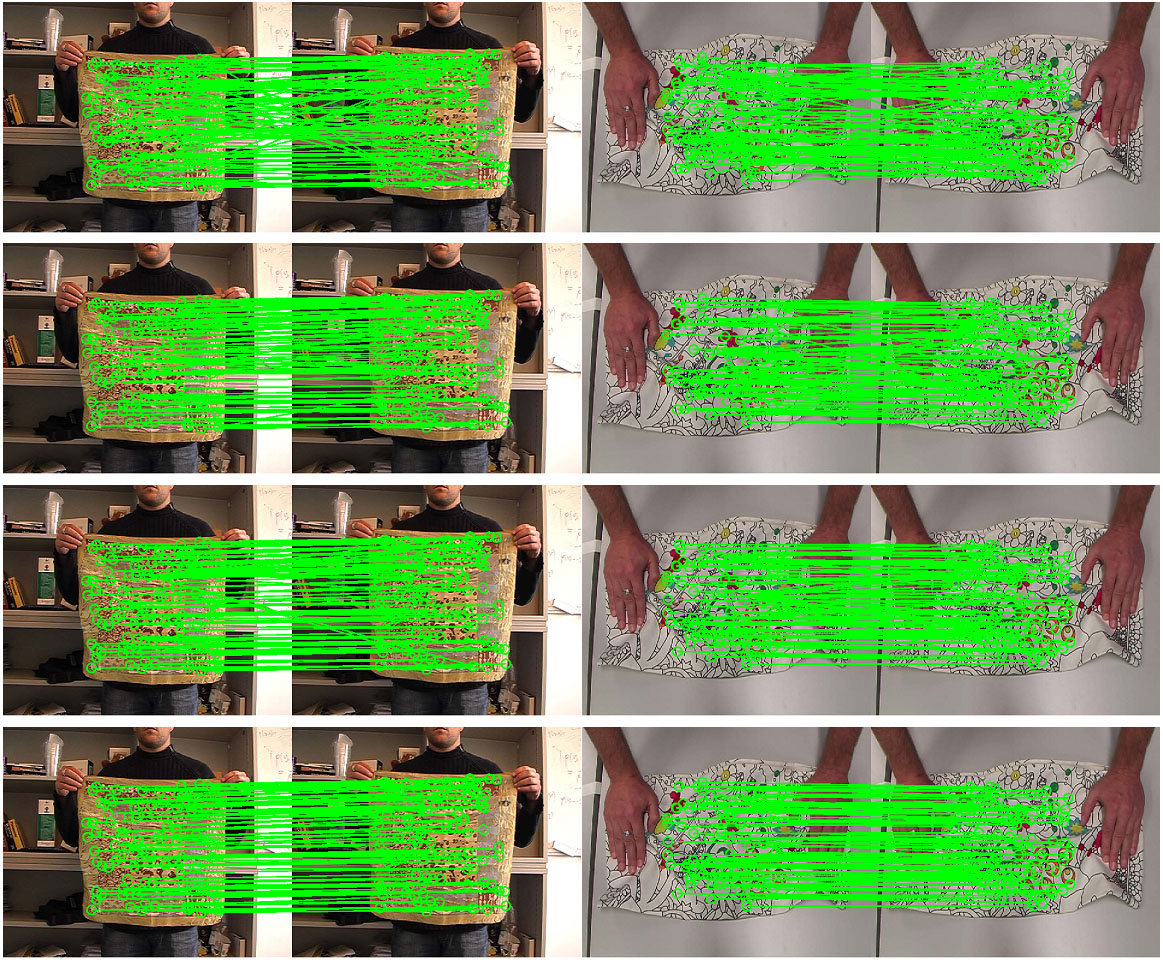
\includegraphics[width=1.05\linewidth]{figures/2DDeformable.jpg}
  \caption{Matching results. Left: cloth set, selected from frame 85 to 110, right: cushion set, selected from frames 144 to 213.
  Top to bottom, spectral method [Cour et al. 2006], hyper graph matching method [Zass and Shashua 2008], a Third-order tensor [Duchenne et al. 2009], and our SuperMatching algorithm.}
\label{fig:2DDeformable}
\end{figure}

%----------------------------------------
%  deformable matching results TABLE
%----------------------------------------
\begin{table}
%\vspace{-4mm}
\centering
%\renewcommand{\arraystretch}{0.8}
\tabcolsep=1pt
\setlength{\aboverulesep}{0pt}
\setlength{\belowrulesep}{0pt}
\caption{Error rate of deformable surface matching.}
\hspace{-5ex}
\label{tab:errorrate1}
\small
\begin{tabular}{l|c c c c | c c c c | c c}
\toprule
{Dataset}  & \multicolumn{4}{|c|}{ {cloth}} & \multicolumn{4}{c|}{ {cushion}} & & \\
\hline
 {Matching frames} &  {F80-}	&  {F90-}	& {F95-}	& {F100-} & {F144-} & {F156-}	& {F165-}	& {F172-} & {Feature}	& {Time}  \\
 {}                &  {F90 }    &  {F95 }   & {F100}    & {F105}  & {F156}  & {F165}    & {F172}    & {F188}  & {Tuples}    &  {(s)} \\
\hline
 {SuperMatching}   &  {17\%}    &  {15\%}	& {16\%} 	& {19\%}  & {34\%}	& {40\%}	& {31\%}	& {44\%}  &  {20k}	    &  {8}  \\
%\hline
 {\cite{Zass08}}   & {27\%}	    & {21\%}	& {30\%}	& {28\%}  & {56\%}  & {61\%}    & {46\%}	& {57\%}   & {40k}	    & {6.5}  \\
%\hline
{\cite{Duchenne09}} & {33\%}    & {23\%}    & {27\%}	& {35\%}  & {61\%}	& {69\%}	& {53\%}	& {58\%}   & {1010k}    & {13}  \\
%\hline
 {\cite{Cour06}}   & {73\%}     & {71\%}	&  {78\%}	& {73\%}  & {86\%}  & {95\%}	& {72\%}	& {93\%}   & {--}       & {5}  \\
\bottomrule
\end{tabular}%
%\vspace{-27pt}
%\vspace{-8mm}
\end{table}%
%

%-------------------------------------------------------------------------
\subsection{3D rigid object scans}
\label{subsec:3DRigid}

\begin{figure}
\centering
  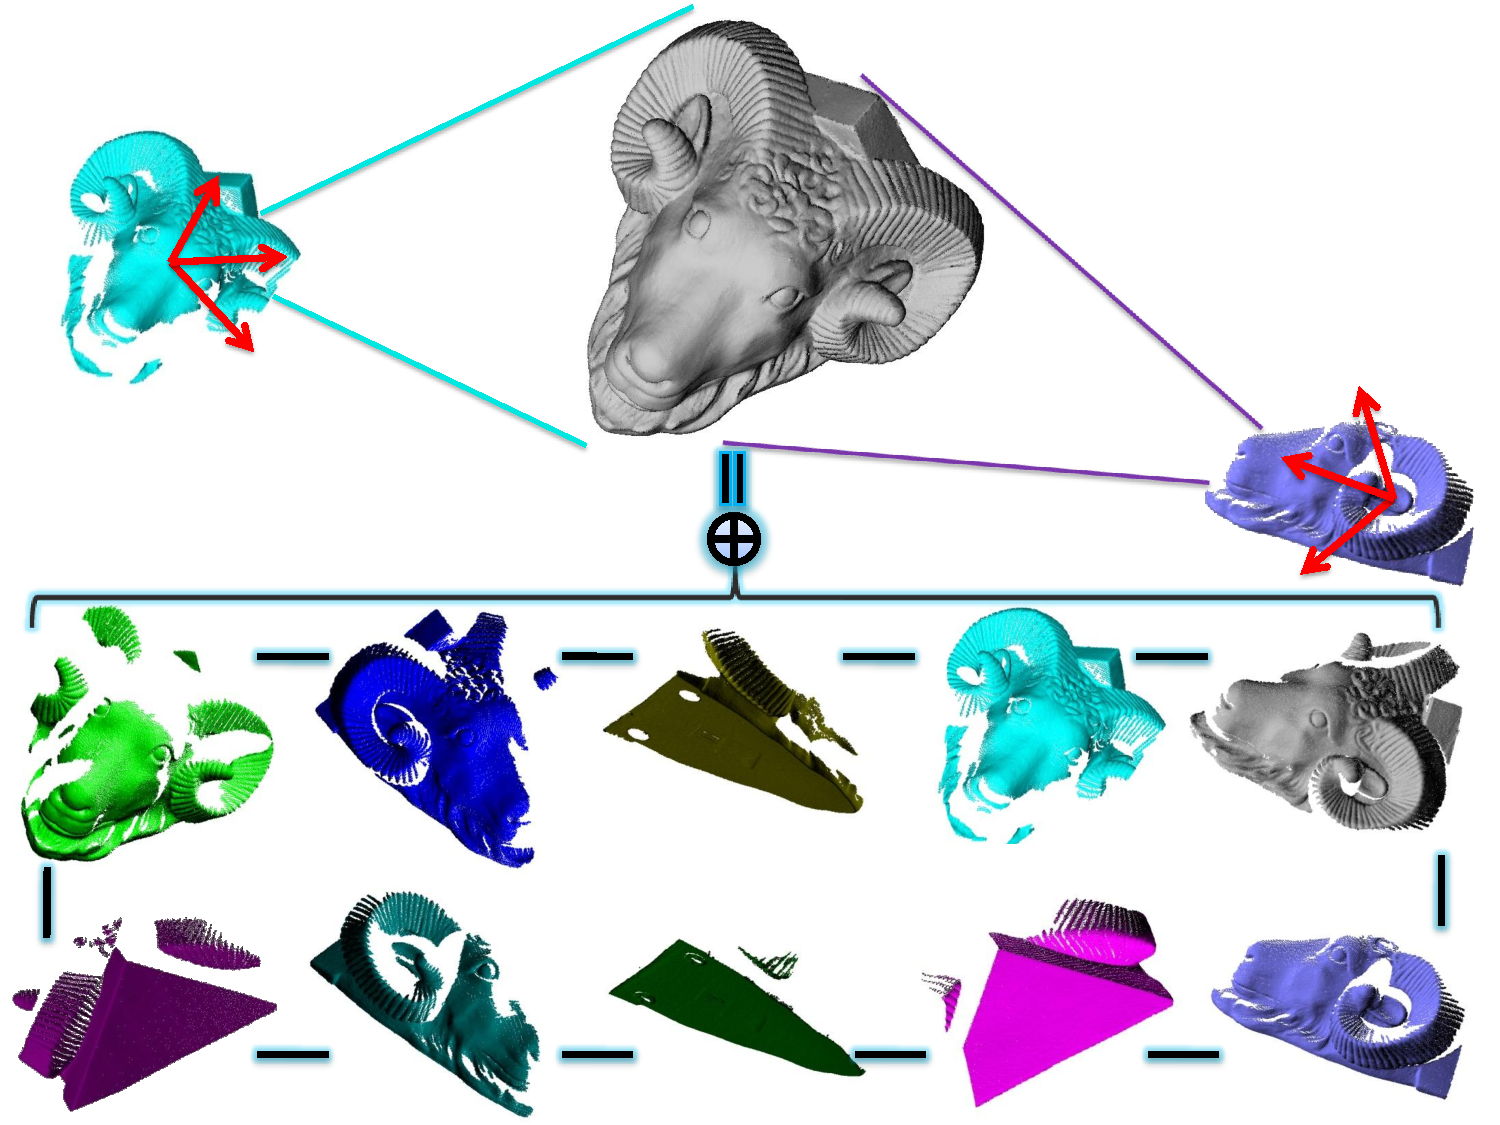
\includegraphics[width=1.0\linewidth]{figures/3DRigid.pdf}
  \caption{Third-order potential schematic diagram. The geometric constraints: internal angle invariance in 2D (up), and edge length invariance in 3D case (bottom).}
\label{fig:3DRigid}
\end{figure}

%-------------------------------------------------------------------------
\subsection{3D articulated object scans}
\label{subsec:3darticulated}

%-------------------------------------------------------------------------
\subsection{3D colorful object scans}
\label{subsec:3dColored}
